\RequirePackage{plautopatch}
\documentclass[uplatex, a4paper, dvipdfmx]{jsarticle}
\usepackage[backend=biber, style=alphabetic, sorting=nyt]{biblatex}
\addbibresource{../bib/double-affine-braid-group.bib} 

\usepackage{amsthm}
\usepackage{amsmath,amsfonts,amssymb}
\usepackage{tikz-cd}
\usepackage{dynkin-diagrams}

\renewcommand{\labelenumi}{(\arabic{enumi})}

\theoremstyle{definition}
\newtheorem{theorem}{定理}[section]
\newtheorem{definition}[theorem]{定義}
\newtheorem{proposition}[theorem]{命題}
\newtheorem{lemma}[theorem]{補題}
\newtheorem{corollary}[theorem]{系}
\newtheorem{fact}[theorem]{事実}
\newtheorem{example}[theorem]{例}
\newtheorem{remark}[theorem]{補足}

\DeclareMathOperator{\Hom}{\mathrm{Hom}}
\DeclareMathOperator{\Tor}{\mathrm{Tor}}
\DeclareMathOperator{\CHom}{\mathcal{H}\!\mathit{om}}
\DeclareMathOperator{\CTor}{\mathcal{T}\!\mathit{or}}
\DeclareMathOperator{\Auteq}{\mathrm{Auteq}}
\DeclareMathOperator{\Cone}{\mathrm{Cone}}
\DeclareMathOperator{\ev}{\mathrm{ev}}
\DeclareMathOperator{\id}{\mathrm{id}}
\DeclareMathOperator{\depth}{\mathrm{depth}}
\DeclareMathOperator{\Pic}{\mathrm{Pic}}
\DeclareMathOperator{\MCG}{\mathrm{MCG}}
\DeclareMathOperator{\PMCG}{\mathrm{PMCG}}
\DeclareMathOperator{\RHom}{\mathrm{RHom}}
\DeclareMathOperator{\Ker}{\mathrm{Ker}}
\DeclareMathOperator{\Image}{\mathrm{Im}}
\DeclareMathOperator{\Aut}{\mathrm{Aut}}
\DeclareMathOperator{\Inn}{\mathrm{Inn}}
\DeclareMathOperator{\Out}{\mathrm{Out}}
\DeclareMathOperator{\Supp}{\mathrm{Supp}}
\DeclareMathOperator{\SL}{\mathrm{SL}}
\DeclareMathOperator{\Spec}{\mathrm{Spec}}
\DeclareMathOperator{\Perf}{\mathrm{Perf}}
\DeclareMathOperator{\NS}{\mathrm{NS}}
\DeclareMathOperator{\Ext}{\mathrm{Ext}}
\DeclareMathOperator{\Hilb}{\mathrm{Hilb}}
\DeclareMathOperator{\res}{\mathrm{res}}
\DeclareMathOperator{\Ch}{\mathrm{Ch}}
\DeclareMathOperator{\coh}{\mathrm{coh}}
\DeclareMathOperator{\Ann}{\mathrm{Ann}}



\newcommand{\nc}{\newcommand}

%% Calligraphic letters

\nc{\cF}{{\mathcal{F}}}
\nc{\cG}{{\mathcal{G}}}
\nc{\cH}{{\mathcal{H}}}
\nc{\cJ}{{\mathcal{J}}}
\nc{\cM}{{\mathcal{M}}}
\nc{\cO}{{\mathcal{O}}}
\nc{\cU}{{\mathcal{U}}}
\nc{\cW}{{\mathcal{W}}}

%% Blackboard letters
\nc{\bA}{{\mathbb{A}}}
\nc{\bC}{{\mathbb{C}}}
\nc{\bP}{{\mathbb{P}}}
\nc{\bQ}{{\mathbb{Q}}}
\nc{\bR}{{\mathbb{R}}}
\nc{\bZ}{{\mathbb{Z}}}


%% Fraktur letters
\nc{\fg}{{\mathfrak{g}}}
\nc{\fu}{{\mathfrak{u}}}

% hyperref
\usepackage[urlcolor=blue]{hyperref}


\title{二重アファインブレイド群の作用}
\author{荒井 勇人}
\date{\today}
\begin{document}
\maketitle
\section{二重アファインブレイド群}

\section{I型の場合の写像類群作用の代数的な定義}
\subsection{Artin群}
\begin{definition}
    $l \in \bZ_{\geq 1}$とする。$l \times l$ Coxeter行列とは、$l \times l$正方行列$M = (m_{ij})_{ij}$であって
    \begin{itemize}
        \item $M$は対称行列であり、
        \item 対角成分は全て$1$であり、
        \item それ以外の成分は$\{2, 3, 4, \dots, \infty\}$に値をとる
    \end{itemize}
    ようなものである。Coxeter行列$M$を考えることは以下のCoxeterグラフ(Coxeter--Dynkin図形)$\Gamma$を考えることと等価である。
    \begin{itemize}
        \item $\Gamma$の頂点は$x_1, \dots, x_l$である。
        \item 頂点$x_i$と$x_j$の間に辺があるのは$m_{ij} \geq 3$のとき。
        \item $m_{ij}\geq 4$のとき$x_i$と$_j$の間の辺にラベル$m_{ij}$をつける。
    \end{itemize}
\end{definition}
\begin{definition}
    Coxeter行列$M$(と対応するCoxeterグラフ$\Gamma$)に付随したArtin群$A(\Gamma)$とは、生成元を$t_1, \dots, t_l$とし
    \begin{equation}
        \underbrace{\cdots t_i t_j t_i}_{m_{ij}} = \underbrace{\cdots t_j t_i t_j}_{m_{ij}}, \quad 1 \leq i, j \leq l, m_{ij} < \infty
    \end{equation}
    を関係式として定義される群のことである。

    また$M$と$\Gamma$に付随するCoxeter群$W(\Gamma)$とは、$A(\Gamma)$を関係式$t_i^2=1 \quad(1\leq i\leq l)$で割ってできる群のことである。
\end{definition}
\begin{remark}
    \begin{enumerate}
        \item 有限Coxeter群は完全に分類されている。すなわち、$W(\Gamma)$が有限かつ$\Gamma$が連結になるような$\Gamma$は完全に分類されている。
        \item Weyl群はCoxeter群として実現できる。
    \end{enumerate}
\end{remark}
\begin{example}
    $A_l$型Coxeterグラフ
    \begin{equation}
        \begin{dynkinDiagram}[text style/.style={scale=1.2},
                edge length=1cm,
                labels={1,2,l-1,l},
                label macro/.code={x_{\drlap{#1}}}
            ]A{}
        \end{dynkinDiagram}
    \end{equation}
    に付随するCoxeter群は対称群$S_{l-1}$であり、Artin群は$l-1$本の紐から定まるブレイド群$B_{l-1}$である。
\end{example}
$X$を$\Gamma$の頂点の部分集合とし、$\Gamma_X$を$X$の定める$\Gamma$の充満部分グラフ、$W_X$を$X$の生成する$W(\Gamma)$の部分群、$A_X$を$X$の生成する$A(\Gamma)$の部分群とする。
\begin{theorem}[\cite{MR0240238,MR1475116}]
    自然な群準同型
    \begin{align}
        W(\Gamma_X) & \to W_X \\
        A(\Gamma_X) & \to A_X
    \end{align}
    は同型である。
\end{theorem}

自然な群準同型$\theta \colon A(\Gamma) \to W(\Gamma)$による$t_i$の像を$s_i$とおく。
$w \in W(\Gamma)$に対し$s_1, \dots, s_l$による最短表示$w = s_{i_1} \cdots s_{i_r}$を1つとり$\tau(w) = t_{i_1}\cdots t_{i_r}$とおくと、$\tau$はwell-definedな写像$\tau \colon W(\Gamma) \to A(\Gamma)$を定めることが知られており、これは$\theta$の(群準同型とは限らない?)切断を与える。

\cite{MR0323910}による群$A(\Gamma)$のfundamental element $\Delta = \Delta(A(\Gamma))$とは、以下で定義される元である(\cite{MR1475117}と\cite[Section 2.3]{MR1805936}を参照)。
まず$w_0$を$W(\Gamma)$の(生成元$s_1, \dots, s_l$に関する)最長元、すなわち$s_1, \dots, s_l$で最短表示したときの長さが最も長い元とする。これは一意に定まることが知られている。そして$\Delta = \tau(w_0)$と定義する。
\begin{remark}
    定義より、$\Delta$は$\Gamma$の自己同型からくるような$A(\Gamma)$の自己同型によって不変である。例えば$A_l$型の場合頂点の添字を逆転させるようなinvolutionがあるが、これにより$\Delta(A_l)$は不変である。
\end{remark}

\subsection{$A$型Artin群における関係式}
$A$を$A_l$型Coxeterグラフから定まるArtin群とする。
すなわち生成元を$t_1, \dots, t_l$とし
\begin{align}
    t_it_{i+1}t_i & = t_{i+1}t_it_{i+1} & 1\leq i \leq l-1 \\
    t_it_j        & = t_jt_i            & |i-j|\geq 2
\end{align}
を関係式として定義される群とする。これは$l+1$本の紐から定まるブレイド群に等しい。
また付随するCoxeter群$W$は、$s_1, \dots, s_l$を生成元とし
\begin{align}
    s_i^2          & = 1 & 1\leq i \leq l   \\
    (s_is_{i+1})^3 & = 1 & 1\leq i \leq l-1 \\
    (s_is_j)^2     & = 1 & |i-j|\geq 2
\end{align}
を関係式として定義される群である。これは$s_i$を互換$(i, i+1)$とする対称群$S_{l+1}$に等しい。
\begin{lemma}\label{relation_of_Delta}
    $A$において
    \begin{equation}
        \Delta(A_l)^2 = (t_1 t_2\cdots t_l)^{l+1}
    \end{equation}
    \begin{align}
        \Delta(A_l) & = t_1 (t_2t_1)(t_3t_2t_1)\cdots(t_l\cdots t_2t_1) \\
                    & =(t_1t_2\cdots t_l)\cdots(t_1t_2t_3)(t_1t_2)t_1
    \end{align}
    が成り立つ。
\end{lemma}
\begin{proof}
    \cite[Proposition 2.8]{MR1805936}と\cite[Lemma 3.1]{MR1475117}である。
\end{proof}
\begin{lemma}\label{involution_of_Delta}
    $A$において関係式
    \begin{equation}
        (t_1t_2\cdots t_l)^{l+1} = (t_l\cdots t_2t_1)^{l+1}
    \end{equation}
    が成り立つ。
\end{lemma}
\begin{proof}
    $i \colon W \to W$と$\iota \colon A \to A$をそれぞれ$s_i \mapsto s_{l+1-i}, t_i \mapsto t_{l+1-i}$となるようなinvolutionとする。これは群準同型である。定義より$w_0$は$i$によって不変である。よって$\Delta(A_l)$は$\iota$により不変であり、$\Delta(A_l)^2 = (t_1t_2\cdots t_l)^{l+1}$も$\iota$により不変である。よって\begin{equation}
        (t_1t_2\cdots t_l)^{l+1} = (t_l\cdots t_2t_1)^{l+1}
    \end{equation}
    が成り立つ。
\end{proof}
\begin{lemma}\label{relation_of_Delta_2}
    $A$において関係式
    \begin{equation}
        (t_1t_2\cdots t_l)^{l+1} = t_l\cdots t_2t_1 (t_2 t_3\cdots t_l)^l t_1t_2\cdots t_l
    \end{equation}
    が成り立つ。
\end{lemma}
\begin{proof}
    Lemma \ref{relation_of_Delta}より
    \begin{align}
        (t_1t_2\cdots t_l)^{l+1} & =\Delta(A_l)^2                                                                                         \\
                                 & = (t_1t_2\cdots t_l)\cdots(t_1t_2t_3)(t_1t_2)t_1 \cdot t_1 (t_2t_1)(t_3t_2t_1)\cdots(t_l\cdots t_2t_1) \\
                                 & = (t_1t_2\cdots t_l) \Delta(A_{l-1})^2(t_l\cdots t_2t_1)                                               \\
                                 & =(t_1t_2\cdots t_l) (t_1t_2\cdots t_{l-1})^{l}(t_l\cdots t_2t_1)
    \end{align}
    が成り立つ。
    これにLemma \ref{involution_of_Delta}のinvolution $\iota$を施すと
    \begin{equation}
        (t_l\cdots t_2t_1)^{l+1} = (t_l\cdots t_2t_1) (t_lt_{l-1}\cdots t_2)^{l}(t_1t_2\cdots t_l)
    \end{equation}
    となる。左辺にLemma \ref{involution_of_Delta}を、右辺に$l-1$の場合のLemma \ref{involution_of_Delta}を($t_2, \dots t_l$の生成する$A$の部分群について)用いると
    \begin{equation}
        (t_1t_2\cdots t_l)^{l+1}=(t_l\cdots t_2t_1) (t_2t_3\cdots t_l)^{l}(t_1t_2\cdots t_l)
    \end{equation}
    となる。
\end{proof}
\subsection{穴あきトーラスの写像類群の表示}
$T_n$を$n$個の穴が空いたトーラスとし、$\MCG(T_n)$をその写像類群とする。

\begin{figure}[h]
    \centering
    \begin{displaymath}
        \begin{tikzpicture}[scale=1.2]
            % big square
            \draw[dashed] (0,0)--(11,0);
            \draw[dashed] (0,0)--(0,4);
            \draw[dashed] (0,4)--(11,4);
            \draw[dashed] (11,4)--(11,0);

            % horizontal lines
            \draw[thick] (1, 2)--(3, 2);
            \draw[thick] (3, 2)--(5, 2);

            \draw[thick] (0, 0.5)--(11, 0.5);

            % vertical lines
            \draw[thick] (2, 0)--(2, 4);
            \draw[thick] (10, 0)--(10, 4);

            % punctures
            \draw[dotted, thick] (5+1, 2)--(9-1, 2);
            \foreach \u in {1, 3, 5, 9}
                {
                    \filldraw[white] (\u, 2) circle (2pt);
                    \draw[black] (\u, 2) circle (2pt);
                }

            % notations
            \draw(0, 0.5) node[left]{$b_1$};
            \draw(2, 4) node[above]{$a_1$};
            \draw(10, 4) node[above]{$a_0$};

            \draw(1, 3) node[above]{$\tau_1$};
            \draw(1, 3) to[out=-90,in=135](1.5, 2);
            \draw(3, 3) node[above]{$\tau_2$};
            \draw(3, 3) to[out=-90,in=135](3.5, 2);



        \end{tikzpicture}
    \end{displaymath}
    \caption{$T_n$上の曲線} \label{curves_on_T_n}
\end{figure}

\begin{theorem}[{\cite[Theorem 3.2]{MR1805936}}]
    $\Gamma$を以下のようなCoxeter図形とする。
    \begin{equation}\label{Coxeter_graph}
        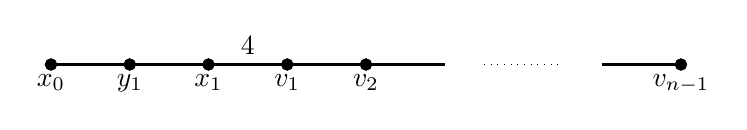
\begin{tikzpicture}
            \foreach \u in {1, 2, 3, 4, 5, 9}
                {
                    \filldraw[black] (\u, 0) circle (2pt);
                    \draw[black] (\u, 0) circle (2pt);
                }
            \draw[thick] (1, 0)--(6, 0);
            \draw[dotted] (6.5, 0)--(7.5, 0);
            \draw[thick] (8, 0)--(9, 0);

            \draw(1, 0) node[below]{$x_0$};
            \draw(2, 0) node[below]{$y_1$};
            \draw(3, 0) node[below]{$x_1$};
            \draw(4, 0) node[below]{$v_1$};
            \draw(5, 0) node[below]{$v_2$};
            \draw(9, 0) node[below]{$v_{n-1}$};

            \draw(3.5, 0) node[above]{$4$};
        \end{tikzpicture}
    \end{equation}
    このとき$\MCG(T_n)$はArtin群$A(\Gamma)$を関係式
    \begin{enumerate}
        \item [(R7)] $(v_1x_1y_1x_0)^4 = (v_1x_1y_1)^6$
        \item [(R9b)] $x_0^n = (x_1 v_1v_2 \cdots v_{n-1})^n$
        \item [(R9c)] $(x_0y_1)^n = (v_1 v_2 \cdots v_{n-1})^n$
    \end{enumerate}
    で割ったものと同型である。
    その同型射は、$v_i$を$\tau_i$に沿った半捻りに、$x_0, y_1, x_2$をそれぞれ$a_0, b_1, a_1$に沿ったDehn捻りにうつすようなものである。
\end{theorem}
\subsection{準備}
$\pi \colon S \to C$を楕円曲面とし、$Y \subset S$をその特異ファイバーとする。

特に断らない限り$Y$は$\textrm{I}_n$型($n \geq 3$)とし、既約成分を順に$G_1, \dots, G_n$とする。
\begin{lemma}
    $Y$は一般の小平ファイバーとし、$L$を$G$上の次数が$0$な直線束とすると、任意の$a$について
    \begin{equation}
        H_{\cO_G(a)}(L) = L
    \end{equation}
    である。
\end{lemma}
\begin{proof}
    $\RHom_S(\cO_G(a), L) = 0$だからよい。
\end{proof}

\begin{proposition}
    $Y$は既約成分が3個以上ある小平ファイバーだとする。
    このとき任意の整数$a$と$Y$の既約成分$G$および直線束$L$について
    \begin{equation}
        (-\otimes L) \circ H_{\cO_G(a)} \circ(- \otimes L)^{-1} = H_{\cO_G(a)\otimes L}
    \end{equation}
    が成り立つ。
\end{proposition}
\begin{proof}
    $L$が$S$上の直線束の制限になっているときには、$H$の定義から直ちに従う。

    以下それ以外の場合を証明する。$Y$の既約成分を$G = G_1, \dots, G_n$とし、$x_i \in G_i$を非特異閉点とする。

    まず$a=-1$と$L = \cO(x_1)$について等式を示す。
    \cite[Lemma 3.3]{MR3182005}の証明と同様にして、等式に$\cO_{x_i}, \cO(x_1)$を代入したときに同型になっていることを確かめればよい。
    $\cO_{x_i}, i \neq 1$については自明である。$\cO(x_1)$についても簡単な計算でわかる。
    $\cO_{x_1}$について、
    \begin{equation}
        LH_{\cO_{G_1}(-1)}(\cO_{x_1}) = H_{\cO_{G_1}}(\cO_{x_1})
    \end{equation}
    を示したい。ここで$S$上の直線束$L'$であって、$L' \cdot G = 1$かつある$G$以外の既約成分とも$0$でない交点数を持つものを1つとる。既約成分が3個以上ある小平ファイバーの場合、$G$とちょうど1点で横断的に交わるような別の既約成分$G'$が存在するので、$L' = \cO_S(G')$とすればよい。既約成分の添字を付け替えて$G' = G_2$とする。
    このとき$L'$の$G_i$上の次数を$d_i$とすると、$d_1 = 1, d_2 \neq 0$であり、
    \begin{equation}
        L_0=L^{-1} \otimes L' \otimes \cO\left(-\sum_{i = 2}^n d_ix_i\right)
    \end{equation}
    は$Y$上の次数$0$の直線束である。$\Pic^0(Y)$は$\bC^*$または$0$と同型だから、$x_2$をうまく取り替えることで$L_0$を自明束にすることができる。(ここで$d_2 \neq 0$を使った。)
    すると
    \begin{align}
        LH_{\cO_{G_1}(-1)}(\cO_{x_1}) & = L' \otimes\cO\left(\sum_{i = 2}^n d_ix_i\right)\otimes H_{\cO_{G_1}(-1)}(\cO_{x_1}) \\
                                      & =L' H_{\cO_{G_1}(-1)}(\cO_{x_1})                                                      \\
                                      & = H_{\cO_{G_1}(-1)\otimes L'}(\cO_{x_1})                                              \\
                                      & =H_{\cO_{G_1}(-1)\otimes L}(\cO_{x_1})
    \end{align}
    となる。ここで2つ目の変形では$-\otimes \cO_{x_i} = T_{\cO_{x_i}}$かつ$x_i (i \neq 1)$が$H_{\cO_{G_1}(-1)}(\cO_{x_1})$の台と交わらないことを使い、3つ目の変形では$S$上の直線束については命題が成り立っていることを使った。

    次に$a=-1$と$L = \cO(x_i), i \neq 1$について示す。示したい等式は
    \begin{equation}
        (-\otimes L) \circ H_{\cO_G(-1)} \circ(- \otimes L)^{-1} = H_{\cO_G(-1)}
    \end{equation}
    となる。上と同様に$\cO_{x_i}, \cO$についての同型を示す。
    $\cO_{X_i}, i \neq 1$については自明である。$\cO(x_1)$についても$x_i (i \neq 1)$が$H_{\cO_{G_1}(-1)}(\cO_{x_1})$の台と交わらないことからわかる。さらに$\cO$についても$\RHom_S(\cO_G(-1), L^{-1}) = 0$となることからわかる。

    以上と$x_i$の取り方が任意なことと$\Pic(Y)$の元はうまく$x_i$を選ぶことで$\cO(\sum_{i}d_ix_i)$の形で表せることを合わせると、$a = -1$と任意の$L$について命題が成り立つ。

    さらに
    \begin{equation}
        H_{\cO_{G_i}(a)} = (- \otimes \cO((a+1)x_i))\circ H_{\cO_{G_i}(-1)} \circ (- \otimes \cO((a+1)x_i))^{-1}
    \end{equation}
    を使うと、他の$a$の場合も$a = -1$に帰着される。
\end{proof}
\begin{proposition}\label{choice_of_x_i}
    (ちょっと怪しい)
    $Y$は既約成分が3個以上の$I$型または$IV$型の小平ファイバーとする。
    $Y$の既約成分を$G_1, \dots, G_n$とし、$d_{ij} = G_i \cdot G_j$とする。
    このとき非特異閉点$x_i \in G_i$を、全ての$i$について
    \begin{equation}
        \cO_S(G_i)\vert_Y \cong \cO_Y\left(\sum_j d_{ij}x_j\right)
    \end{equation}
    となるようにとることができる。

    特に$Y$が$I$型または$IV$型の場合、$\cO_S(G_i)\vert_Y \cong \cO_Y(x_{i-1} - 2x_i + x_{i+1})$となるようにとることができる。
\end{proposition}
\begin{proof}
    $I$型のとき、$(x_i)_i \in (\bC^*)^n$についての方程式
    \begin{equation}
        \cO_S(G_i)\vert_Y \cong \cO_Y(x_{i-1} - 2x_i + x_{i+1})
    \end{equation}
    を考える。
    非特異閉点$y_i \in G_i$を適当に選び、同型
    \begin{equation}
        \{L \in \Pic(Y) \mid \deg L = (\dots, 0, 1, -2, 1, 0, \dots)\} \to \Pic^0(Y), \quad L \mapsto L \otimes \cO(-y_{i-1}+2y_i-y_{i+1})
    \end{equation}
    を使うと、
    \begin{equation}
        \varphi \colon (\bC^*)^n \to (\Pic^0(Y))^n, \quad (x_i)_i \mapsto \cO(x_{i-1}-y_{i-1} - 2(x_i-y_i)+x_{i+1}-y_{i+1})
    \end{equation}
    の像が$(\cO_S(G_i) \otimes \cO(-y_{i-1}+2y_i-y_{i+1}))_i$を含むことを示せばよいことになる。
    そのためには$\varphi$の像が
    \begin{equation}
        \{(L_i)_i \in (\Pic^0(Y))^n \mid L_1 \otimes \cdots \otimes L_n = \cO\}
    \end{equation}
    になることを示せば十分である。像がこの部分集合に含まれることはわかる。同型$\Pic^0(Y) \cong \bC^*$より、この集合は$\Ker((\bC^*)^n \to \bC^*) \cong (\bC^*)^{n-1}$と(代数群として)同一視される。$\varphi$は多様体の射だから、$\Image \varphi$の次元が$n-1$であることを示せば十分である。具体的に計算することで$\varphi\vert_{(\bC^*)^{n-1} \times 1 }$のファイバーが$n(n-1)$点集合であることからわかり、よって$\Image \varphi$は$n-1$次元である。

    $IV$型のときは$\bC^*$を$\bC$に置き換えて全く同じ議論をすればよい。この場合は$\varphi$が単射になる。
\end{proof}
\begin{definition}\label{conjugate_action}
    $Y$が既約成分を3個以上持つ小平ファイバーのとき、$L_i = - \otimes \cO(x_i), H_i = H_{\cO_{G_i}(-1)}, T = T_\cO \in \Auteq D^b(Y)$とする。
    $Y$が$I$または$IV$型のときはProposition \ref{choice_of_x_i}のように$x_i$を選ぶこととする。
\end{definition}

\begin{proposition}\label{HLHL}
    $Y$が既約成分を3個以上持つ小平ファイバーのとき、全ての$i$について
    \begin{equation}
        H_iL_iH_iL_i = L_iH_iL_iH_i = -\otimes \cO_S(G_i)\vert_Y \otimes L_i^2
    \end{equation}
    が成り立つ。特に$Y$が$I$型または$IV$型なら
    \begin{equation}
        H_iL_iH_iL_i = L_iH_iL_iH_i = L_{i-1}L_{i+1}
    \end{equation}
    となる。
\end{proposition}
\begin{proof}
    まずProposition \ref{conjugate_action}より$L_iH_iL_i^{-1}=H_{\cO_{G_i}}$と$L_i^{-1}H_iL_i=H_{\cO_{G_i}(-2)}$が成り立つ。
    よって$L_i^{-1}H_iL_iH_i = H_{\cO_{G_i}(-2)} \circ H_{\cO_{G_i}(-1)}$および$H_iL_iH_iL_i^{-1} = H_{\cO_{G_i}(-1)} \circ H_{\cO_{G_i}}$がわかる。
    さらに\cite[Lemma3.15]{MR2198807}より$T_{\cO_{G_i}(a-1)}\circ T_{\cO_{G_i}(a)} = - \otimes \cO_S(G_i)$だから、図式
    \begin{equation}
        \begin{tikzcd}
            D^b(Y) \arrow[r,"i_*"]\arrow[d, "H_{\cO_{G_i}(a-1)}\circ H_{\cO_{G_i}(a)}"'] & D^b(S) \arrow[d,"T_{\cO_{G_i}(a-1)}\circ T_{\cO_{G_i}(a)}= - \otimes \cO_S(G_i)"]\\
            D^b(Y) \arrow[r, "i_*"]& D^b(S).
        \end{tikzcd}
    \end{equation}
    を可換にするという一意性から$H_{\cO_{G_i}(a-1)}\circ H_{\cO_{G_i}(a)} = - \otimes \cO_S(G_i)\vert_Y$がわかる。
    以上より
    \begin{equation}
        L_i^{-1}H_iL_iH_i =H_iL_iH_iL_i^{-1} = \otimes \cO_S(G_i)\vert_Y
    \end{equation}
    となり命題が従う。
\end{proof}
\subsection{Artin群関係式}
$Y$は既約成分が$3$個以上ある小平ファイバーとする。
\begin{proposition}\label{Artin_relation}
    $\Auteq D^b(Y)$において、以下の関係式が成り立つ。
    \begin{align}
        TL_iT        & = L_iTL_i \label{eq:01}                                        \\
        L_iL_j       & = L_jL_i \label{eq:02}                                         \\
        H_iL_j       & = L_jH_i                     & i \neq j \label{eq:03}          \\
        H_iT         & = TH_i \label{eq:04}                                           \\
        H_iL_iH_iL_i & = L_iH_iL_iH_i \label{eq:05}                                   \\
        H_iH_{j}H_i  & = H_{j}H_iH_{j}              & G_i \cdot G_j = 1 \label{eq:06} \\
        H_iH_j       & = H_jH_i                     & G_i \cdot G_j = 0 \label{eq:07}
    \end{align}
\end{proposition}
\begin{proof}
    \eqref{eq:01}は捻り関手のブレイド関係式である。\eqref{eq:02}は自明。\eqref{eq:03}は$H_i(\cO_{x_j}) = \cO_{x_j}$またはProposition \ref{conjugate_action}から従う。\eqref{eq:04}は$H_i(\cO) = \cO$から従う。\eqref{eq:05}はProposition \ref{HLHL}である。\eqref{eq:06}と\eqref{eq:07}は$S$における捻り関手$T_{\cO_{G_i}(-1)}$のブレイド関係式の帰結である。
\end{proof}
以下では$Y$は$I_n$型($n \geq 3$)または$IV$型の小平ファイバーとする。さらに既約成分の添字$i$は巡回的にとるものとする。

\begin{corollary}\label{Artin_relation_cor}
    $\Gamma$を\eqref{Coxeter_graph}のようなCoxeter図形とし、$A(\Gamma)$を付随するArtin群とすると、群準同型$A(\Gamma) \to \Auteq D^b(Y)$であって
    \begin{align}
        x_0 = x_n & \mapsto L_0 = L_n                   \\
        y_1       & \mapsto T                           \\
        x_1       & \mapsto L_1                         \\
        v_i       & \mapsto H_i, \quad 1\leq i \leq n-1
    \end{align}
    となるものがある。すなわち以下の関係式が成り立つ。
    \begin{align}
        TL_0T         & = L_0TL_0 \label{eq:1}                                      \\
        L_1L_0        & = L_1L_0 \label{eq:2}                                       \\
        H_iL_0        & = L_0H_i                    & 1\leq i \leq n-1 \label{eq:3} \\
        L_1TL_1       & = TL_1T \label{eq:4}                                        \\
        H_iT          & = TH_i                      & 1\leq i \leq n-1 \label{eq:5} \\
        H_1L_1H_1L_1  & = L_1H_1L_1H_1 \label{eq:6}                                 \\
        H_iH_{i+1}H_i & = H_{i+1}H_iH_{i+1}         & 1\leq i \leq n-2 \label{eq:7} \\
        H_iH_j        & = H_jH_i                    & |i-j|>1\label{eq:8}
    \end{align}
\end{corollary}


\subsection{R7}
\begin{proposition}[R7]
    $Y$が$I$または$IV$型のとき
    \begin{equation}
        (H_1L_1TL_0)^4 = (H_1L_1T)^6
    \end{equation}
    が成り立つ。
\end{proposition}
\begin{proof}
    Proposition \ref{Artin_relation}を使って変形すると
    \begin{align}
        (H_1L_1TL_0)^4 & =H_1L_1T \cdot L_0 \cdot H_1L_1TL_0 \cdot H_1L_1TL_0 \cdot H_1L_1TL_0 \\
                       & =(H_1L_1T) \cdot H_1L_1L_0TL_0 \cdot H_1L_1TL_0 \cdot H_1L_1TL_0      \\
                       & =(H_1L_1T) \cdot H_1L_1TL_0T \cdot H_1L_1TL_0 \cdot H_1L_1TL_0        \\
                       & =(H_1L_1T) \cdot H_1L_1T \cdot L_0TH_1L_1TL_0 \cdot H_1L_1TL_0        \\
                       & =(H_1L_1T)^2 \cdot H_1\cdot L_0TL_1TL_0 \cdot H_1L_1TL_0              \\
                       & =(H_1L_1T)^2 \cdot H_1\cdot L_0L_1TL_1L_0 \cdot H_1L_1TL_0            \\
                       & =(H_1L_1T)^2 \cdot H_1\cdot L_1L_0TL_0L_1 \cdot H_1L_1TL_0            \\
                       & =(H_1L_1T)^2 \cdot H_1\cdot L_1TL_0TL_1 \cdot H_1L_1TL_0              \\
                       & =(H_1L_1T)^3 \cdot L_0TL_1 \cdot H_1L_1TL_0                           \\
    \end{align}
    となるから、$L_0TL_1H_1L_1TL_0=(H_1L_1T)^3$を示せばよい。
    右辺はProposition \ref{HLHL}の$I$または$IV$型のときの主張を使うと
    \begin{align}
        (H_1L_1T)^3 & = H_1L_1T \cdot H_1L_1T \cdot H_1L_1T   \\
                    & = H_1L_1H_1 \cdot TL_1T \cdot H_1L_1T   \\
                    & = H_1L_1H_1 \cdot L_1TL_1 \cdot H_1L_1T \\
                    & = H_1L_1H_1L_1\cdot TL_1 \cdot H_1L_1T  \\
                    & = L_0L_2\cdot TL_1 \cdot H_1L_1T
    \end{align}
    だから、両辺に$L_0^{-1}$を左からかけた$TL_1H_1L_1TL_0=L_2 TL_1 H_1L_1T$を示せばよい。
    両辺に左から$H_1$をかけると左辺は
    \begin{align}
        H_1TL_1H_1L_1TL_0 & = TH_1L_1H_1L_1T \\
                          & = TL_0L_2TL_0    \\
                          & = TL_2L_0TL_0    \\
                          & = TL_2TL_0T
    \end{align}
    で、右辺は
    \begin{align}
        H_1L_2TL_1H_1L_1T & = L_2TH_1L_1H_1L_1T \\
                          & = L_2TL_0L_2T       \\
                          & = L_2TL_2L_0T       \\
                          & = TL_2TL_0T
    \end{align}
    となって等しいから、$TL_1H_1L_1TL_0=L_2 TL_1 H_1L_1T$が成り立つ。
\end{proof}
\subsection{R9b}
\begin{proposition}[R9b]
    $Y$が$I$または$IV$型のとき
    \begin{equation}
        L_0^n = (L_1H_1\cdots H_{n-1})^n
    \end{equation}
    が成り立つ。
\end{proposition}
\begin{proof}
    $i = 2, 3, \dots, n$に対して$A_i = L_0^{1-i}(L_1H_1\cdots H_{i-1})^i$とおく。
    帰納法で$A_i = L_i$を示す。$i=2$のときはProposition \ref{HLHL}よりよい。
    帰納法とProposition \ref{HLHL}より、$A_{i-1}A_{i+1} = H_iA_iH_iA_i$が成り立つことを示せばよい。
    これは\cite[Theorem 3.8]{MR1805936}の証明と全く同様。
\end{proof}
\subsection{R9c'}
ここでは$Y$は$I$または$IV$型とする。
\begin{lemma}\label{cohomology_on_type_4}
    $Y$が$IV$型の曲線のとき、
    \begin{equation}
        H^0(L_0L_1^{-1}L_2) = \bC, \quad H^1(L_0L_1^{-1}L_2) = 0
    \end{equation}
    である。
\end{lemma}
\begin{proof}
    $\pi \colon \widetilde{Y} = \coprod_{i = 1}^3 \bP^1_i \to Y$を正規化とする。
    また$\cO = \cO_Y, \widetilde{\cO} = \cO_{\widetilde{Y}}$とし、$\cJ = \Ann_{\cO}(\pi_*\widetilde{\cO}/\cO)$を導手、$\iota \colon S = V(\cJ) \to Y$を$\cJ$が定める$Y$の閉部分スキーム、$\widetilde{\iota} \colon \widetilde{S} \to \widetilde{Y}$をそのスキーム論的逆像とする。
    \begin{equation}
        \begin{tikzcd}
            \widetilde{S} \arrow[r, "\widetilde{\iota}"]\arrow[d, "\widetilde{\pi}"]& \widetilde{Y}\arrow[d, "\pi"]\\
            S \arrow[r, "\iota"]& Y
        \end{tikzcd}
    \end{equation}
    \cite{MR1872612}によると、このとき$Y$上のランク$r$のベクトル束は以下のデータと等価である。
    \begin{itemize}
        \item $\widetilde{Y}$上のランク$r$のベクトル束$\widetilde{\cG}$
        \item $S$上の(ランク$r$の)自明束$\cM$
        \item 同型射$\widetilde{\mu}
                  \colon \widetilde{\pi}^*\cM \to \widetilde{\cG}\vert_{\widetilde{S}}$
    \end{itemize}
    これらのデータが与えられたとき、$Y$上の対応するベクトル束$\cG$は以下のようにして構成される。
    まず$\widetilde{\mu}$の誘導する射
    \begin{equation}
        \mu \colon \iota_*\cM=G \to \iota_*\widetilde{\pi}_*(\widetilde{\cG}\vert_{\widetilde{S}})=F
    \end{equation}
    を考える。これは単射である。そして$\cG$は以下の引き戻しで定まる層である。
    \begin{equation}
        \begin{tikzcd}
            \cG \arrow[r]\arrow[d] & \iota_*\cM = G \arrow[d]\\
            \pi_*\widetilde{\cG} \arrow[r] & \iota_*\widetilde{\pi}_*(\widetilde{\cG}\vert_{\widetilde{S}}) = F
        \end{tikzcd}
    \end{equation}
    これにより$L_0L_1^{-1}L_2$に対応するデータは以下のようになる。
    \begin{itemize}
        \item $\widetilde{\cG} = \cO_1(-1)\oplus\cO_2(1)\oplus\cO_3(1)$
        \item $\cM = \cO_S$
        \item $\widetilde{\mu} \colon \widetilde{\pi}^*\cM \cong \cO_{\widetilde{S}} \to \cO_{\widetilde{S}} \cong \widetilde{\cG}\vert_{\widetilde{S}}$
    \end{itemize}
    よって$H = F/G$とおくと、$\cG = L_0L_1^{-1}L_2$は以下の完全列で特徴づけられる。
    \begin{equation}
        0 \to \cG \to \pi_*\widetilde{\cG} \to H \to 0
    \end{equation}
    ここで$Y$の唯一の特異点$s$の周りでの座標を$Y = \Spec \bC[x, y]/xy(x-y)$ととり、$\bP^1_i$の斉次座標を$[z_{i0} : z_{i1}]$、非斉次座標を$t_i = z_{i0}/z_{i1}$とし、$\pi$を
    \begin{equation}
        \begin{tikzcd}
            \bC[x, y]/xy(x-y) \arrow[r]& \bigoplus_{i=1}^3 \bC[t_i] \\
            x \arrow[r, mapsto] & (t_1, t_2, 0) \\
            y \arrow[r, mapsto] & (t_1, 0, t_3)
        \end{tikzcd}
    \end{equation}
    と表示する。すると$\cO_S = \bC[x,y]/(x^2, y^2, xy), \cO_{\widetilde{S}} = \bigoplus_{i=1}^3 \bC[t_i]/(t_i^2) = \bigoplus_{i=1}^3 \bC[\varepsilon_i]$となる。
    そして$\widetilde{\mu} \colon \bigoplus_{i=1}^3 \bC[\varepsilon_i] \to \bigoplus_{i=1}^3 \bC[\varepsilon_i]$は適切に同型で取り替えることによって
    \begin{equation}
        \widetilde{\mu} = (1_1 + \lambda \varepsilon_1, 1_2, 1_3) = 1 + \lambda \varepsilon_1
    \end{equation}
    ととれる。ただし$\lambda \in k$は次数$0$の直線束に対応するパラメータである。
    そして$\mu \colon G \to F = \bigoplus_{i=1}^3 \bC[\varepsilon_i]$の像は
    \begin{equation}
        \varepsilon_1 + \varepsilon_2, \varepsilon_1 + \varepsilon_3, 1 + \lambda \varepsilon_1
    \end{equation}
    で生成される部分層となる。
    よって
    \begin{equation}
        H = F/G = \bigoplus_{i=1}^3 \bC[\varepsilon_i]/(k(\varepsilon_1 + \varepsilon_2) + k( \varepsilon_1 + \varepsilon_3) + k(1 + \lambda \varepsilon_1))
    \end{equation}
    であり、$\cG = L_0L_1^{-1}L_2$のコホモロジーは以下の長完全列を満たす。
    \begin{align}
        0 & \to H^0(\cG) \to H^0(\pi_*\widetilde{\cG}) \to H \\
          & \to H^1(\cG) \to H^1(\pi_*\widetilde{\cG})\to 0
    \end{align}
    $\widetilde{\cG}$の定義より$H^0(\pi_*\widetilde{\cG}) = \bC z_{20} \oplus \bC z_{21}\oplus \bC z_{30}\oplus \bC z_{31}, H^1(\pi_*\widetilde{\cG}) = 0$だから、$H^0(\pi_*\widetilde{\cG}) \to H$が全射であることを示せば命題が従う。その像は
    \begin{equation}
        1_2, \varepsilon_2, 1_3, \varepsilon_3
    \end{equation}
    で生成されるから、$H$の定義から全射となる。
\end{proof}
\begin{lemma}\label{image_of_ox}
    $1\leq i < j \leq n-1$のとき
    \begin{align}
        H_i^{-1}\cdot\cdots \cdot H_{j-1}^{-1}(\cO_{x_{j-1}}) & = T_{L_{i-1}^{-1}L_i}T^{-1}(\cO_{x_j}) = \Cone(L_{i-1}^{-1}L_i \to L_j)          \\
        H_i\cdot\cdots \cdot H_{j-1}(\cO_{x_{j-1}})           & = T_{L_{i-1}L_i^{-1}}^{-1}T(\cO_{x_j})[-1] = \Cone(L_j^{-1} \to L_{i-1}L_i^{-1})
    \end{align}
    が成り立つ。
\end{lemma}
\begin{proof}
    1つ目のみ示す。2つ目も同様である。添字の名前を変えて$i=1$としてよい。$j$で帰納法をする。

    $j=2$のとき\cite[Theorem 2.2]{MR2025266}とLemma \ref{cohomology_on_type_4}より$H^0(L_0L_1^{-1}L_2) = \bC, H^1(L_0L_1^{-1}L_2) = 0$だから、
    \begin{align}
        T_{L_0^{-1}L_1}T^{-1}(\cO_{x_2}) & =L_0^{-1}L_1T(L_0L_1^{-1}L_2)                                               \\
                                         & =L_0^{-1}L_1 \Cone(\RHom(\cO, L_0L_1^{-1}L_2)\otimes\cO \to L_0L_1^{-1}L_2) \\
                                         & =L_0^{-1}L_1 \Cone(\cO \to L_0L_1^{-1}L_2)                                  \\
                                         & = \Cone(L_0^{-1}L_1 \to L_2)
    \end{align}
    となり、$L_0^{-1}L_1 \to L_2$は$0$でない射である。
    さらに$H_1(L_2) = L_2$および
    \begin{align}
        H_1(L_0^{-1}L_1) & = H_1 (\cO(G_1)^{-1}L_1^{-1}L_2)             \\
                         & =H_1(H_{\cO_{G_1}(-2)}H_1)^{-1}(L_1^{-1}L_2) \\
                         & =H_{\cO_{G_1}(-2)}(L_1^{-1}L_2)              \\
                         & =L_1^{-1}L_2
    \end{align}
    が成り立つ(これは球面対象と台が交わらないことによる)。
    よって\begin{align}
        H_1T_{L_0^{-1}L_1}T^{-1}(\cO_{x_2}) & = \Cone(H_1(L_0^{-1}L_1) \to H_1(L_2)) \\
                                            & =\Cone(L_1^{-1}L_2 \to L_2)
    \end{align}
    となり、$L_1^{-1}L_2 \to L_2$は$0$でない射だからその$\Cone$は$\cO_{x_1}$に等しい。

    $j \geq 3$のとき、帰納法の仮定と$j=2$のときと同様の議論を使うと
    \begin{align}
        H_1^{-1}\cdot\cdots \cdot H_{j-1}^{-1}(\cO_{x_{j-1}}) & = H_1^{-1}\Cone(L_{1}^{-1}L_2 \to L_j) \\
                                                              & =\Cone(L_{0}^{-1}L_1 \to L_j)          \\
                                                              & =T_{L_0^{-1}L_1}T^{-1}(\cO_{x_j})
    \end{align}
    となる。
\end{proof}
\begin{lemma}
    $1 \leq j \leq n-1$のとき
    \begin{equation}
        H_1 \cdots H_{j-1}L_{j-1}H_{j-1} \cdots H_1 = L_0L_1^{-1}L_j
    \end{equation}
    が成り立つ。
\end{lemma}
\begin{proof}
    $j$で帰納法をする。$j=1$ならば自明である。またProposition \ref{HLHL}と帰納法の仮定より
    \begin{align}
        H_1 \cdots H_{j-1}H_jL_{j}H_jH_{j-1} \cdots H_1 & =H_1 \cdots H_{j-1}(L_{j-1}L_j^{-1}L_{j+1})H_{j-1}\cdots H_1 \\
                                                        & =H_1 \cdots H_{j-1}L_{j-1}H_{j-1} \cdots H_1 L_j^{-1}L_{j+1} \\
                                                        & =L_0L_1^{-1}L_jL_j^{-1}L_{j+1}                               \\
                                                        & =L_0L_1^{-1}L_{j+1}
    \end{align}
    となりよい。
\end{proof}

\begin{lemma}\label{recurrence_formula_for_Phi}
    $1\leq i \leq j \leq n$に対し$\Phi_{i,j} = (H_i \cdots H_{j-1})^{j-i+1}\in \Auteq D^b(Y)$とおくと、
    \begin{equation}
        \Phi_{i, j} = L_{i-1}L_i^{-1}L_j T_{H_i^{-1}\cdots H_{j-1}^{-1}(\cO_{x_j})}^{-1} \cdot \Phi_{i+1, j}
    \end{equation}
    が成り立つ。
\end{lemma}
\begin{proof}
    $i=1$として示す。
    \begin{align}
         & L_{0}L_1^{-1}L_j T_{H_1^{-1}\cdots H_{j-1}^{-1}(\cO_{x_j})}^{-1} \cdot \Phi_{2, j}                                                             \\
         & =H_1 \cdots H_{j-1}L_{j-1}H_{j-1}\cdots H_1 \cdot H_1^{-1}\cdots H_{j-1}^{-1} L_{j-1}^{-1}(H_1^{-1}\cdots H_{j-1}^{-1})^{-1} \cdot \Phi_{2, j} \\
         & =H_1 \cdots H_{j-1} \cdot(H_1^{-1}\cdots H_{j-1}^{-1})^{-1} \cdot \Phi_{2, j}                                                                  \\
         & =H_1 \cdots H_{j-1} \cdot H_{j-1}\cdots H_1 \cdot (H_2 \cdots H_{j-1})^{j-1}
    \end{align}
    だから、命題は
    \begin{equation}
        (H_1 \cdots H_{j-1})^j=H_1 \cdots H_{j-1} \cdot H_{j-1}\cdots H_1 \cdot (H_2 \cdots H_{j-1})^{j-1}
    \end{equation}
    となる。これはさらに
    \begin{equation}
        (H_1 \cdots H_{j-1})^{j-1}=H_{j-1}\cdots H_1 \cdot (H_2 \cdots H_{j-1})^{j-1}
    \end{equation}
    \begin{equation}
        (H_1 \cdots H_{j-1})^j=H_{j-1}\cdots H_1 \cdot (H_2 \cdots H_{j-1})^{j-1}\cdot H_1 \cdots H_{j-1}
    \end{equation}
    と同値だが、最後の等式はLemma \ref{relation_of_Delta_2}である。
\end{proof}
\begin{proposition}[R9c']
    $(L_0T)^n = (H_1\cdots H_{n-1})^n[2]$
\end{proposition}
\begin{proof}
    $E_{i, j} = L_{i}L_i^{-1}L_{j+1} T_{H_{i+1}^{-1}\cdots H_{j}^{-1}(\cO_{x_{j+1}})}$とおくと、Lemma \ref{recurrence_formula_for_Phi}より
    \begin{equation}
        (H_1 \cdots H_{n-1})^n = E_{0, n-1}E_{1, n-1}\cdots E_{n-2, n-1}
    \end{equation}
    が成り立つ。
    さらにLemma \ref{image_of_ox}より
    \begin{align}
        E_{i, j} & = L_{i}L_{i+1}^{-1}L_{j+1} T_{H_{i+1}^{-1}\cdots H_{j}^{-1}(\cO_{x_{j+1}})}^{-1}                                                                                \\
                 & =L_{i}L_{i+1}^{-1}L_{j+1} \cdot T_{T_{L_i^{-1}L_{i+1}} T^{-1}(\cO_{x_{j+1}})}^{-1}                                                                              \\
                 & = L_{i}L_{i+1}^{-1}L_{j+1} \cdot (L_i^{-1}L_{i+1} T L_{i+1}^{-1}L_i \cdot T^{-1}) \cdot L_{j+1}^{-1}\cdot (L_i^{-1}L_{i+1} T L_{i+1}^{-1}L_i \cdot T^{-1})^{-1} \\
                 & = L_{j+1}T^{-1} L_{i+1}^{-1}L_i T^{-1}L_{j+1}^{-1}TL_i^{-1}L_{i+1}T^{-1}L_{i+1}^{-1}L_i
    \end{align}
    となり、これは\cite[Theorem 3.6]{MR3182005}の証明の中の$E_{i,j}$と等しい。
    さらに\cite[Theorem 3.6]{MR3182005}の証明より($IV$型でも)
    \begin{equation}
        (TL_0)^6 = E_{0, n-1}E_{1, n-1}\cdots E_{n-2, n-1}[2]
    \end{equation}
    が成り立つから、以上を合わせると
    \begin{equation}
        (L_0T)^n = (H_1\cdots H_{n-1})^n[2]
    \end{equation}
    を得る。
\end{proof}
\begin{corollary}\label{H^2}
    $\Auteq D^b(Y)$において関係式
    \begin{align}
        H_1^2 & = L_0L_1^{-1}L_2T_{L_0^{-1}L_1}T^{-1}L_2^{-1}T T_{L_0^{-1}L_1}^{-1} \\
              & =T_{L_0L_1^{-1}}^{-1}TL_2^{-1}T^{-1}T_{L_0L_1^{-1}}L_0L_1^{-1}L_2
    \end{align}
    が成り立つ。
\end{corollary}
\begin{proof}
    1つ目の式はLemma \ref{recurrence_formula_for_Phi}とLemma \ref{image_of_ox}からわかる。2つ目も同様。
\end{proof}
\subsection{結論}
\cite{MR1805936}によると、$n$点穴あきトーラスの写像類群はArtin群$A(\Gamma)$をR7, R9b, R9cで割ったものである。
R9cの代わりにR9c'を使って得られる$\MCG(T_n)$の$\bZ$中心拡大を$\widetilde{\MCG}(T_n)$とおくと、以上の議論により$Y$が$I$型または$IV$型のとき群準同型\begin{equation}
    \widetilde{\MCG}(T_n) \to \Auteq D^b(Y)
\end{equation}
が得られる。

\section{楕円ブレイド群の作用}
\begin{definition}
    $n$点の楕円ブレイド群$B^{Ell}_n$を、トーラス上の$n$点の配置空間の基本群として定義する。\cite{MR2507111}によると、これは以下の生成元と関係式で表される。

    生成元は$X_1, \dots, X_n, Y_1, \dots, Y_n, T_1, \dots, T_{n-1}$で、$X_i$たちは可換、$Y_i$たちは可換、$T_i$たちはブレイド関係式
    \begin{align}
        T_iT_{i+1}T_i & = T_{i+1}T_iT_{i+1} & 1\leq i \leq l-1 \\
        T_iT_j        & = T_jT_i            & |i-j|\geq 2
    \end{align}
    を満たし、さらに関係式
    \begin{align}
        T_iX_iT_i        & = X_{i+1}                                                      & 1\leq i \leq n-1 \label{eq:a} \\
        T_iY_iT_i        & = Y_{i+1} \label{eq:b}                                         & 1\leq i \leq n-1              \\
        T_1^2X_1Y_2      & = Y_2X_1\label{eq:c}                                                                           \\
        \widetilde{Y}X_i & = X_i\widetilde{Y},\quad\widetilde{Y} = \prod_{i = 1}^{n-1}Y_i & 1\leq i \leq n \label{eq:d}
    \end{align}
    が成り立つ。
\end{definition}
\begin{remark}
    \cite{MR2507111}では\eqref{eq:c}の代わりに
    \begin{equation}
        X_1Y_2 = Y_2X_1T_1^2
    \end{equation}
    が使われているが、これらは基本群での演算の順序を逆にすることで等価となる。
    後述するように写像類群との関係を見る上では\eqref{eq:c}を使うような演算の記法の方がわかりやすい。
\end{remark}
\begin{proposition}
    自然な群準同型$B^{Ell}_n \to \MCG(T_n)$は
    \begin{equation}
        B^{Ell}_n \to \widetilde{\MCG}(T_n)
    \end{equation}
    に持ち上がる。
\end{proposition}
\begin{theorem}
    $Y$が$I$型または$IV$型のとき群準同型$B^{Ell}_n \to \Auteq D^b(Y)$で
    \begin{align}
        X_i & \mapsto T_{L_0^{-1}L_{i-1}}^{-1}T_{L_0^{-1}L_i} = L_0^{-1}L_{i-1}T^{-1}L_{i-1}^{-1}L_iTL_0L_i^{-1} \\
        Y_i & \mapsto L_{i-1}^{-1}L_i                                                                            \\
        T_i & \mapsto H_i
    \end{align}
    となるようなものが存在する。
\end{theorem}
\begin{proof}
    関係式\eqref{eq:a}、\eqref{eq:b}、\eqref{eq:c}、\eqref{eq:d}を確かめればよい。
    まず$\prod_{i=1}^{n-1} L_{i-1}^{-1}L_i = 1$だから\eqref{eq:d}は自明である。
    また\eqref{eq:b}はLemma \ref{HLHL}から直ちに従う。

    \eqref{eq:a}を示す。同値変形を繰り返すと
    \begin{align}
        H_i(L_0^{-1}L_{i-1}T^{-1}L_{i-1}^{-1}L_iTL_0L_i^{-1})H_i   & = L_0^{-1}L_{i}T^{-1}L_{i}^{-1}L_{i+1}TL_0L_{i+1}^{-1}     \\
        L_0^{-1}H_i(L_{i-1}T^{-1}L_{i-1}^{-1})(L_iTL_i^{-1})H_iL_0 & = L_0^{-1}(L_{i}T^{-1}L_{i}^{-1})(L_{i+1}TL_{i+1}^{-1})L_0 \\
        H_i(L_{i-1}T^{-1}L_{i-1}^{-1})(L_iTL_i^{-1})H_i            & = (L_{i}T^{-1}L_{i}^{-1})(L_{i+1}TL_{i+1}^{-1})            \\
        H_i(T^{-1}L_{i-1}^{-1}T)(T^{-1}L_iT)H_i                    & = (T^{-1}L_{i}^{-1}T)(T^{-1}L_{i+1}T)                      \\
        H_i(T^{-1}L_{i-1}^{-1}L_iT)H_i                             & = T^{-1}L_{i}^{-1}L_{i+1}T                                 \\
        T^{-1}(H_iL_{i-1}^{-1}L_iH_i)T                             & = T^{-1}L_{i}^{-1}L_{i+1}T                                 \\
        H_iL_{i-1}^{-1}L_iH_i                                      & =L_{i}^{-1}L_{i+1}
    \end{align}
    となりLemma \ref{HLHL}に帰着する。ここで1つ目と3つ目の変形ではCorollary \ref{Artin_relation_cor}のArtin群関係式を使った。

    最後に\eqref{eq:c}を示す。関係式を$T_1^2 = Y_2X_1Y_2^{-1}X_1^{-1}$と変形する。Corollary \ref{H^2}より、$\Auteq D^b(Y)$において左辺は
    \begin{equation}
        L_0L_1^{-1}L_2 \cdot T_{L_0^{-1}L_1}T^{-1}\cdot L_2^{-1} \cdot T T_{L_0^{-1}L_1}^{-1}
    \end{equation}
    となり、$X_1 \mapsto T^{-1}T_{L_0^{-1}L_1} = T_{L_0^{-1}L_1}T^{-1}$だから右辺は
    \begin{equation}
        L_1^{-1}L_2 \cdot T_{L_0^{-1}L_1}T^{-1} \cdot L_1L_2^{-1} \cdot T T_{L_0^{-1}L_1}^{-1}
    \end{equation}
    となる。よって示したい式を同値変形すると
    \begin{align}
        L_0 \cdot T_{L_0^{-1}L_1}T^{-1} & = T_{L_0^{-1}L_1}T^{-1} \cdot L_1 \\
        L_1TL_0L_1^{-1}T^{-1}           & = T^{-1}L_0^{-1}L_1TL_0           \\
        L_1TL_1^{-1}\cdot L_0T^{-1}     & = T^{-1}L_1 \cdot L_0^{-1}TL_0    \\
        T^{-1}L_1T\cdot L_0T            & = T^{-1}L_1 \cdot TL_0T^{-1}      \\
    \end{align}
    となり正しい。ここで最後の変形にはブレイド関係式$ABA = BAB$から従う関係式$ABA^{-1}=B^{-1}AB$を用いた。
\end{proof}


\printbibliography[title=参考文献]
\end{document}